\documentclass[twocolumns]{IEEEtran}
\usepackage{algorithm}
\usepackage{algpseudocode}
\usepackage{graphicx}
\usepackage{caption}
\usepackage{url}
\captionsetup{justification=centering}


\algnewcommand\algorithmicforeach{\textbf{for each}}
\algdef{S}[FOR]{ForEach}[1]{\algorithmicforeach\ #1\ \algorithmicdo}

\author{Erdal Sidal Dogan, Alp Gokcek \\ MEF University \\ \today}
\title{Dijkstra's Shortest Path Algorithm Implementation \& Visualization}


\begin{document}
	\maketitle
	\begin{abstract}
		Dijkstra's Shortest Path Algorithm is an algorithm which finds the shortest path between two nodes in a graph. It is widely used and adopted for many different applications, such as computer networks, road maps, social platforms etc. In this project we implemented algorithm in Python Language and visualized the shortest path.
	\end{abstract}
	\begin{IEEEkeywords}
		Graph, Node, Vertex, Edge
	\end{IEEEkeywords}
	\section{Introduction}
	\textit{Dijkstra's Algorithm} calculates the shortest path from one desired node of the graph to every other nodes. There are varios implementations of the algorithm, main difference between them is how they store the verticies of the graph, denoted with $Q$. They can be stored in regular arrays, linked lists, adjacency lists or tree structures. Running time of the algorithm can be represented with number of edges $|E|$ and number of verticies $|V|$ using big-o notation. Running time mainly depends on these structures, storing $Q$ in arrays it is $\mathcal{O}(|V|^2)$. In this project we utilized the \textit{priority queue} structure while implementing. It is more efficient way to implement comparing to arrays and adjacency lists etc. The \textit{priority queue} implementation requires $\mathcal{O}((|E| + |V|) \log{|V|})$ time in the worst case. 
	\begin{algorithm}
		\caption{Using a priority queue \cite{wiki}}
		\begin{algorithmic}[1]
			\Function {Dijkstra} {\textit{Graph, source}}
				\ForEach {vertex \textbf{v} in \textit{Graph}}
					\State $dist[v] \leftarrow$ INFINITY                  
					\State $prev[v] \leftarrow$ UNDEFINED
					\State add v to Q                      
				\EndFor
				\State $dist[source] \leftarrow$ 0
	
				\While {$Q$ is not empty}
					\State $u \leftarrow$ vertex in $Q$ with min $dist[u]$
					\State remove $u$ from $Q$
					\ForEach {neighbor $v$ of $u$}
						\State $alt \leftarrow dist[u] + length(u, v)$
						\If{alt $<$ dist[v]}
							\State $dist[v] \leftarrow alt$
							\State $prev[v] \leftarrow u$
						\EndIf
					\EndFor
				\EndWhile \\
				\Return dist[], prev[]
			\EndFunction
		\end{algorithmic}
	\end{algorithm}

	\section{The Program}
	\begin{center}
		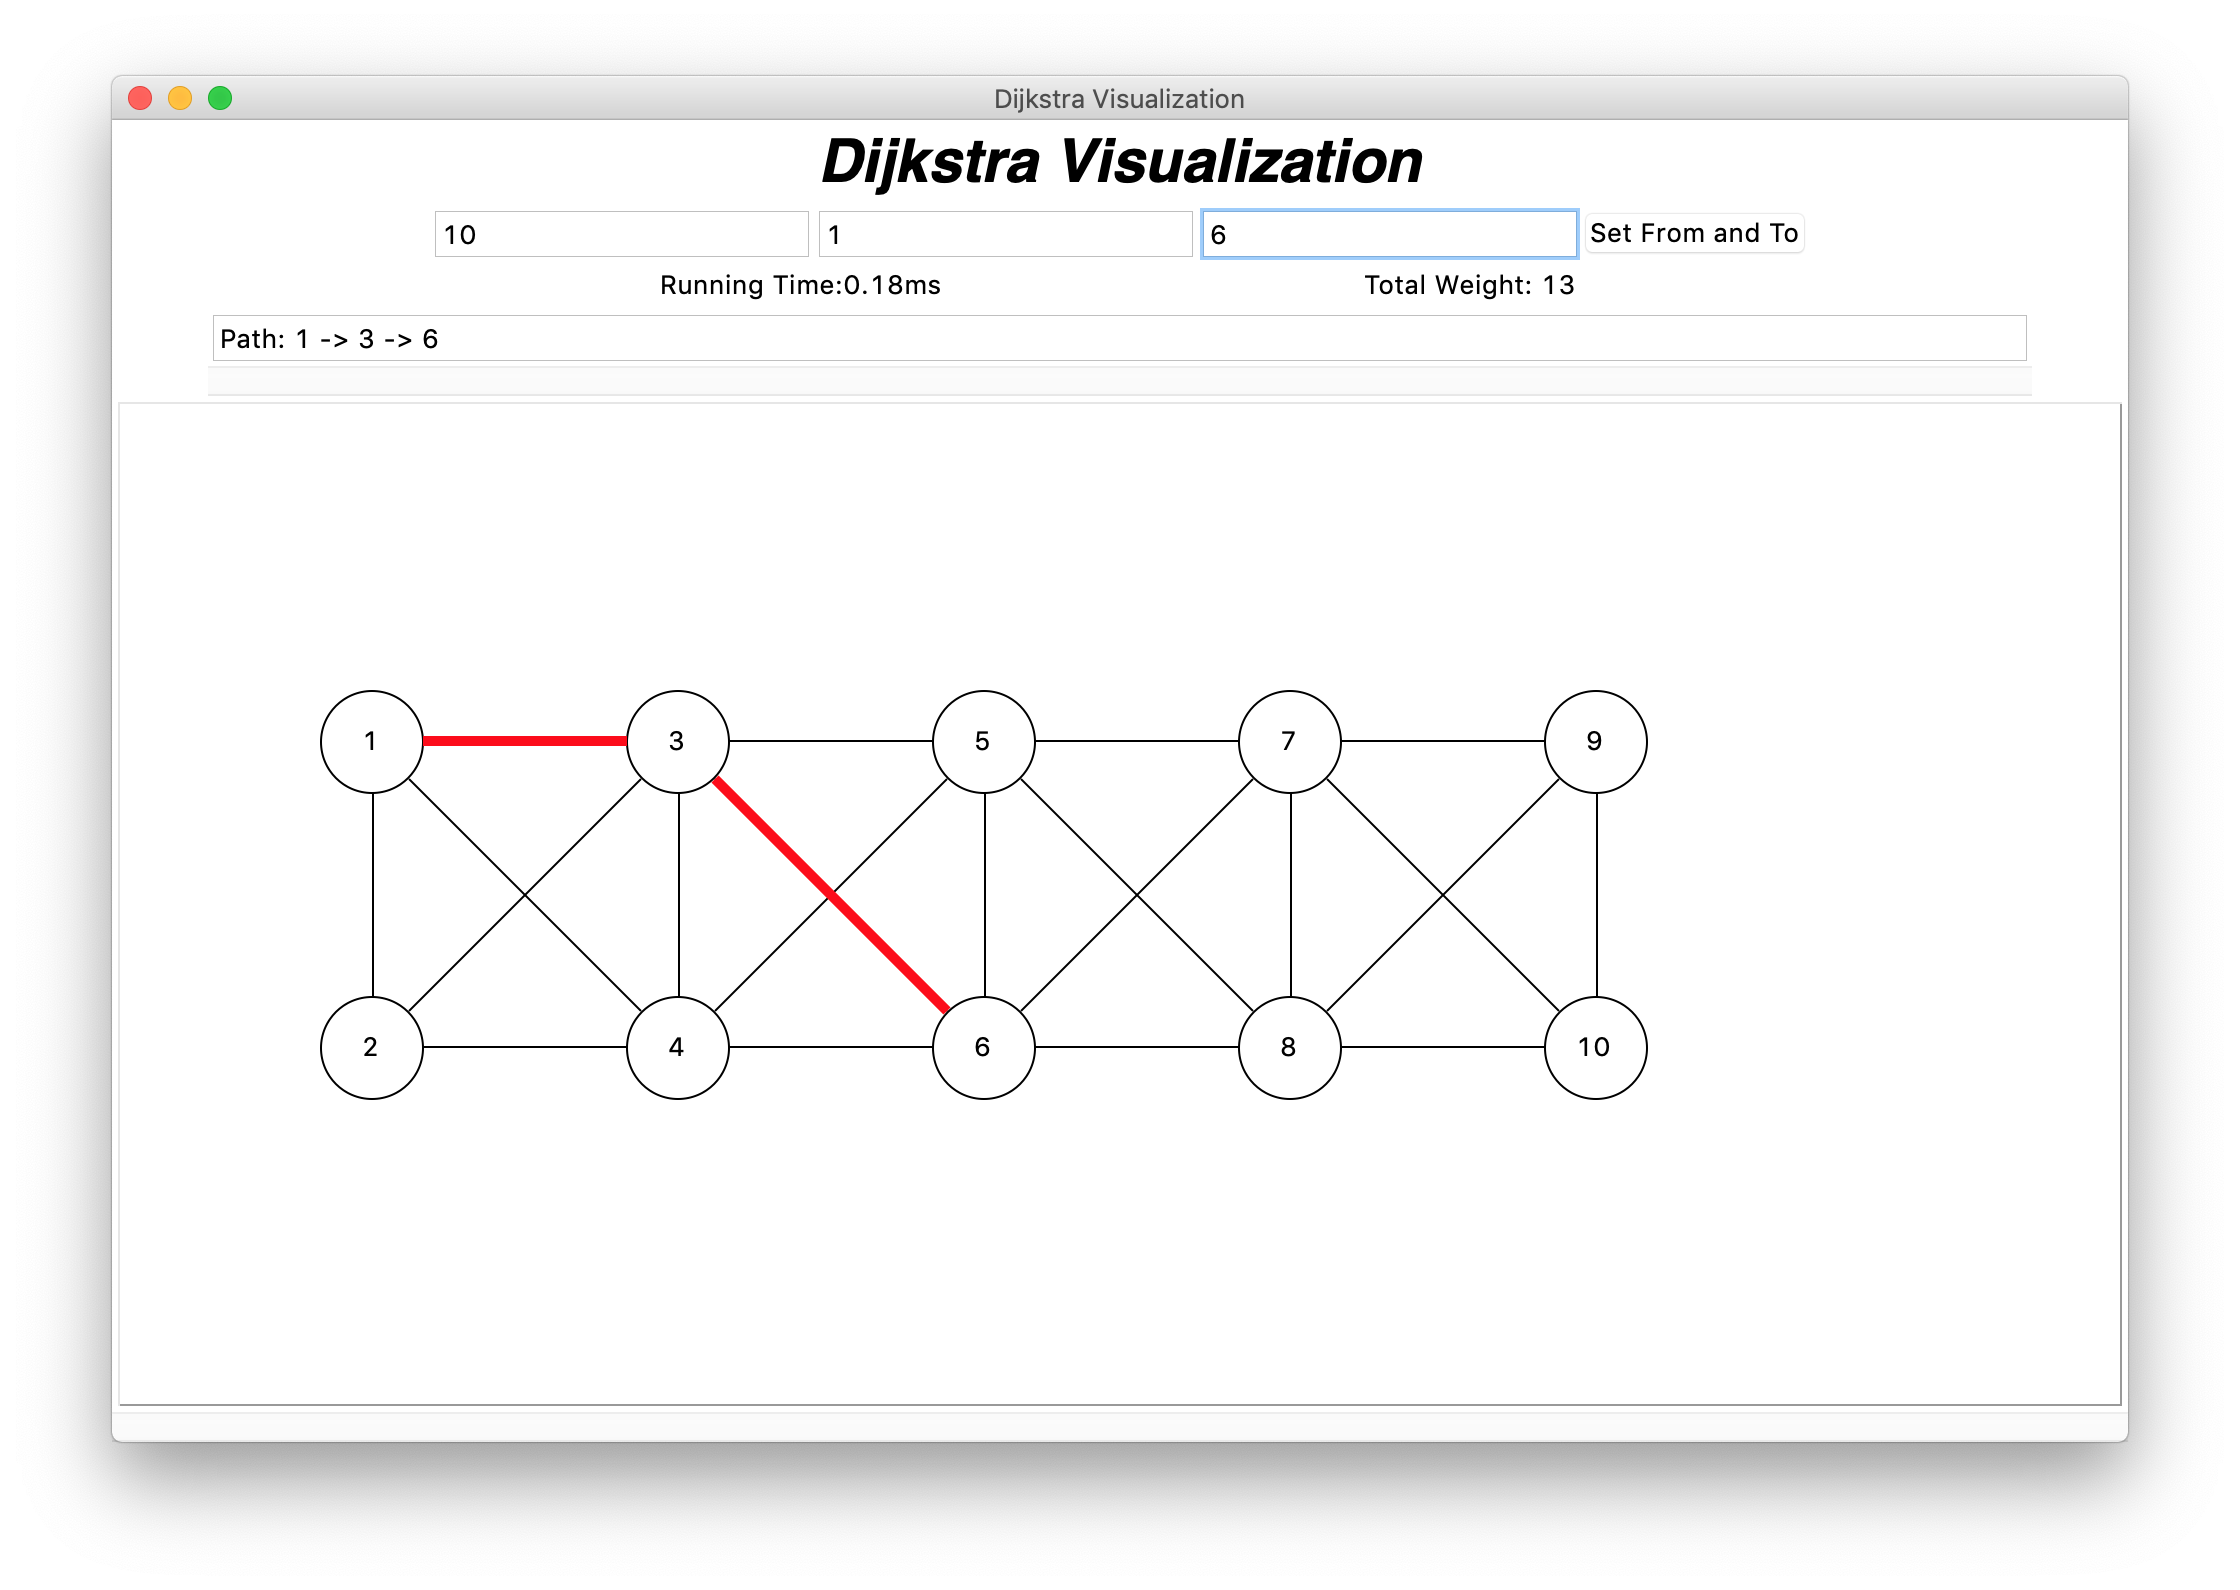
\includegraphics[scale=.2]{main_window.png}
	\end{center}
	\captionof{figure}{Main Window of the program for values selected as; N=10, S=1, D=6}
	
	\section{Time Meausurements}
	\begin{figure}[h]
		\centering
		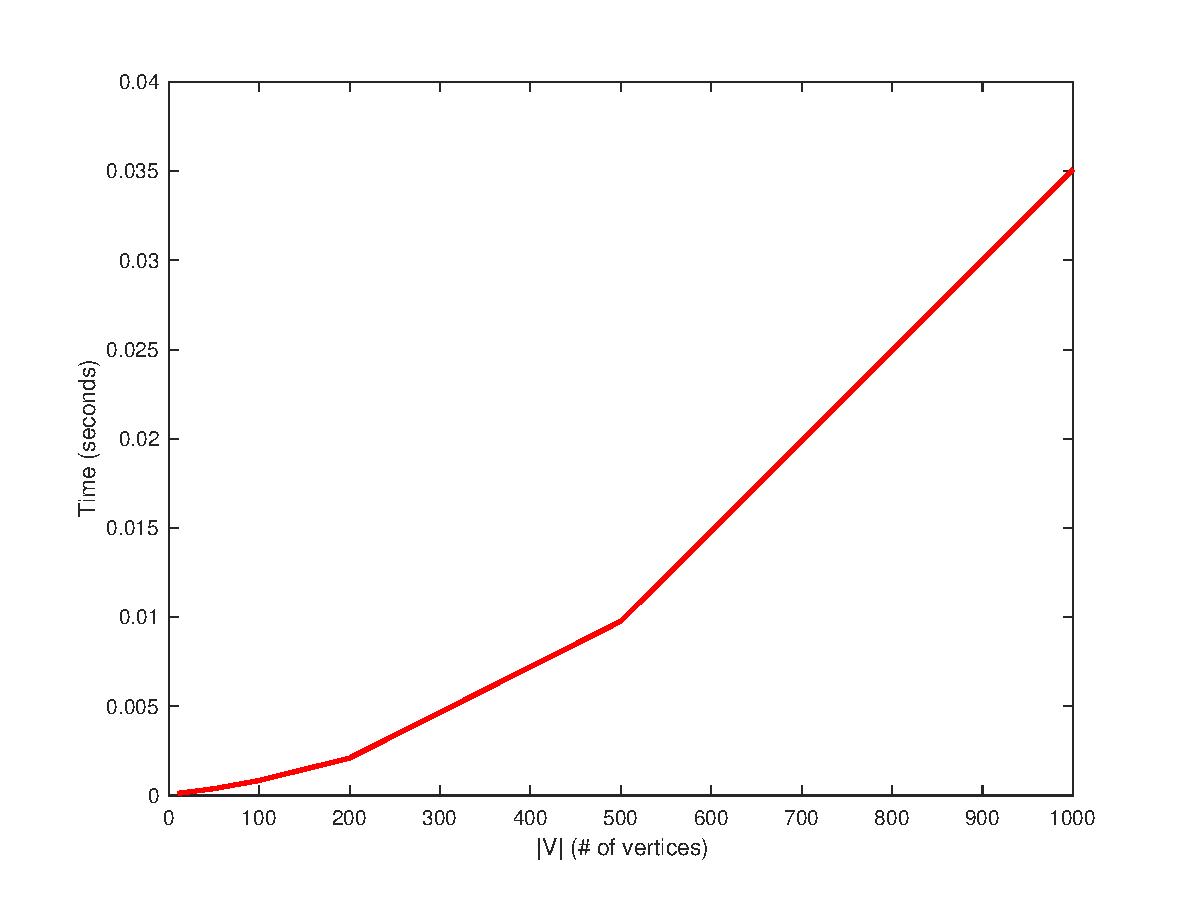
\includegraphics[scale=.4]{matlab/time.eps}
	\end{figure}

	\bibliographystyle{IEEEtran}
	\bibliography{references}

\end{document}